\section{Exercise 3: Architecture}

\begin{figure}[h!]
    \caption{Database layer diagram (updated)}
    \centering
    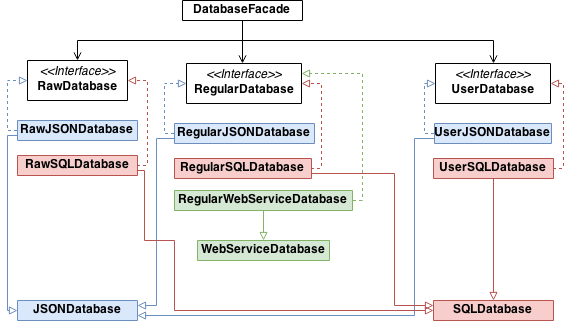
\includegraphics[width=0.8\textwidth]{images/database.png}
\end{figure}

The UML diagram shown above is an updated version from the diagram used in the
2nd assignment. The \hl{WebServiceDatabase} and \hl{RegularWebServiceDatabase}
were added (in green). \hl{DatabaseFacade} instantiates a \hl{UserDatabase},
\hl{RawDatabase} and \hl{RegularDatabase} with the help of the
\hl{DatabaseFactoryProducer} class. This class instantiates the 3 correct
database classes based on the chosen type of database (JSON or SQL). What was
added in this assignment is the instantiation of a \hl{RegularWebServiceDatabase}.
So, a new database layer was added and no modification to the 3-tier architecture
was needed.

\newpage
